\section{Experimental Results}
\label{sec:results}
\subsection{Overall classification performance}
Table~\ref{tab:results} compares the validation-selected checkpoints.
Validation accuracy describes the 6,000-image selection partition; test
accuracy describes the separate 10,000-image official test partition.
All test metrics refer to the same ordered images.

\begin{table}[H]\centering
\caption{Results of the five saved runs. Accuracy is a percentage;
macro-F1 is on the 0--1 scale. Epoch is selected by validation loss.}
\label{tab:results}
\small
\begin{tabular}{lrrrrrr}\toprule
Model & Epoch & Val.\ acc. & Test acc. & Test F1 & Test loss & Errors\\\midrule
\tabledata{generated/results_rows.tex}
\bottomrule\end{tabular}
\end{table}

The CNN has the highest test accuracy and macro-F1, and the lowest test loss.
Its 91.94\% accuracy is 3.44 percentage points above the MLP and 7.68 points above
the Linear model. Relative to the MLP, it reduces the number of mistakes from
1,150 to 806, a reduction of 344 images or 29.9\% of the MLP's errors.

The MLP improves over Linear by 4.24 percentage points. Adding nonlinear hidden
layers is therefore useful in this experiment, even though both models use the
same flattened input. The CNN improves further while retaining spatial
neighborhoods, but its larger capacity also changes the comparison.

\begin{figure}[H]\centering
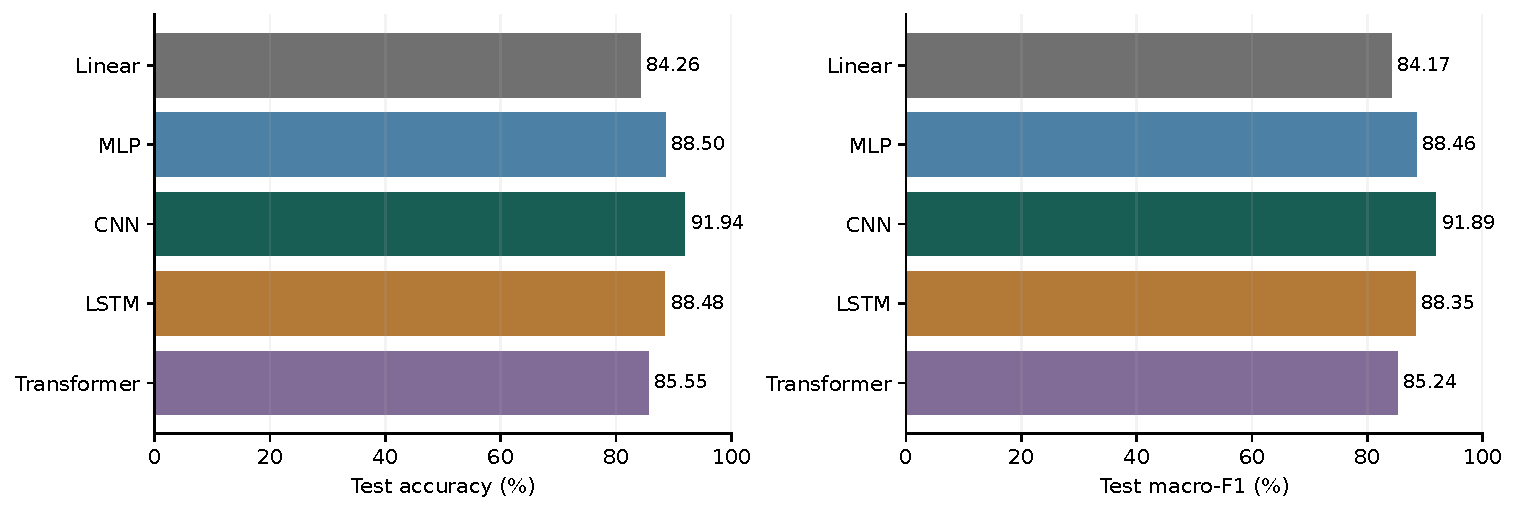
\includegraphics[width=\linewidth]{test_comparison.pdf}
\caption{Official-test accuracy and macro-F1, both displayed as percentages.
Axes start at zero. These are single-run scores, without repeated-seed error bars.}
\label{fig:comparison}
\end{figure}

MLP and LSTM are almost tied: their test accuracies differ by 0.02 percentage
points, or two images. This is too small to support a stable ranking without
repeated runs. Their macro-F1 values are also close, although their class-level
mistakes differ.

The Transformer obtains 85.55\% test accuracy, 1.29 percentage points above
Linear and below the other nonlinear models. This result describes the small,
two-block patch model trained for ten epochs. It does not establish that
attention-based image models are generally weaker than CNNs or MLPs.

Because the test set has equal class support, weighted F1 and macro-F1 are
identical here. Accuracy and macro-F1 remain different measures: F1 also
depends on how false positives are distributed across classes.

\clearpage
\subsection{Learning behavior and checkpoint selection}
Figure~\ref{fig:curves} shows the recorded training and validation losses for
all ten epochs. The same vertical scale is used for every model.

\begin{figure}[H]\centering
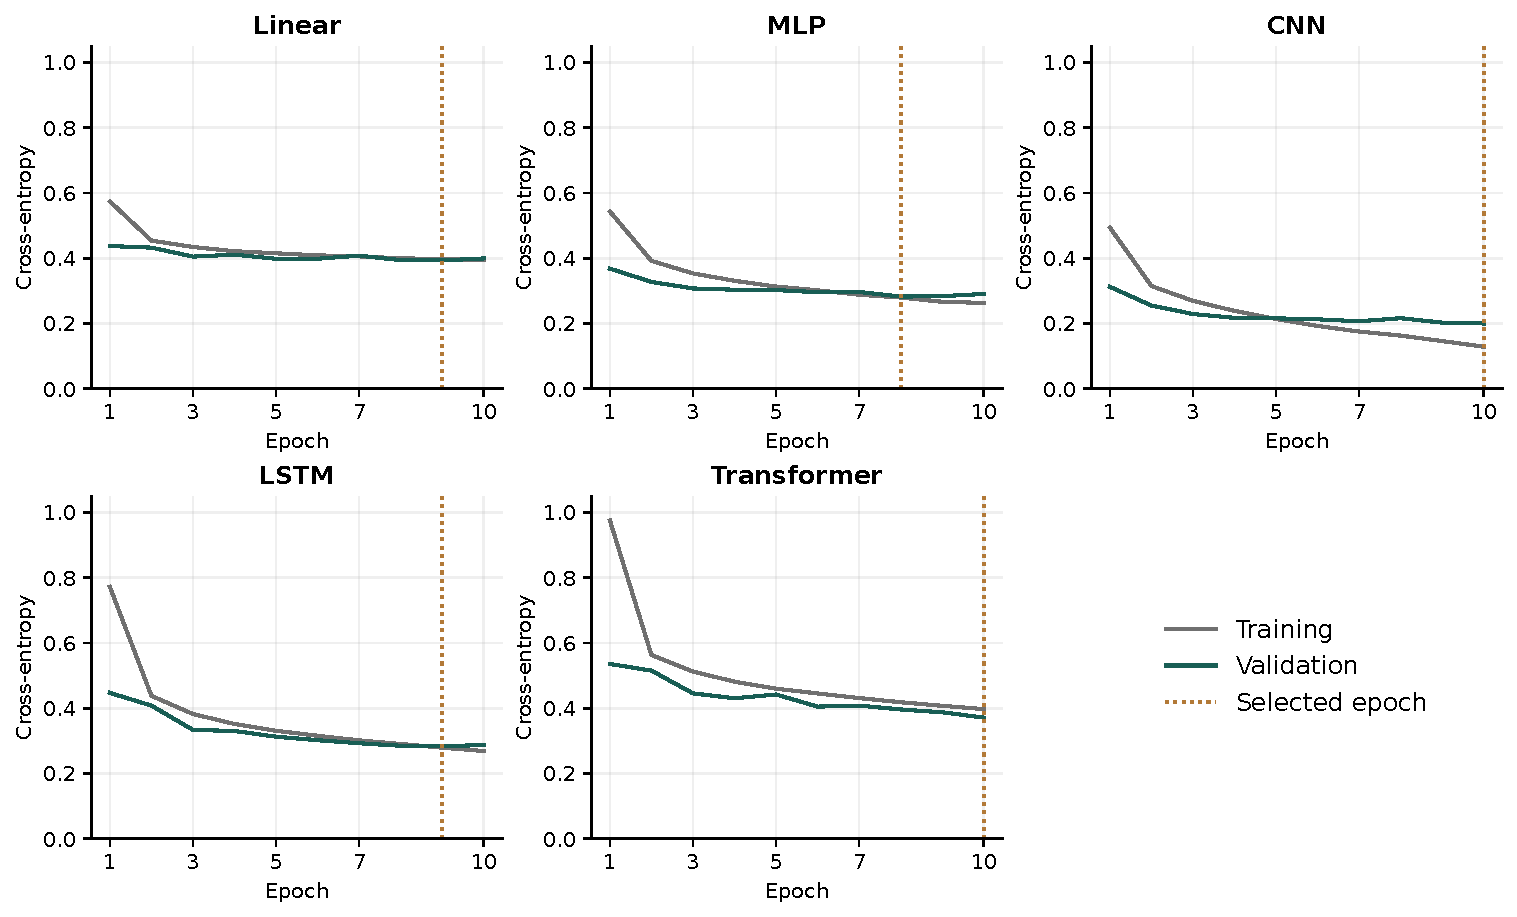
\includegraphics[width=\linewidth]{learning_curves.pdf}
\caption{Cross-entropy over ten epochs. Dotted lines mark the checkpoint with
the lowest validation loss. Training loss is collected with dropout active
and changing weights; validation loss uses evaluation mode after each epoch.}
\label{fig:curves}
\end{figure}

\begin{table}[H]\centering
\caption{First and final validation losses, with final-epoch accuracies.
These final-epoch values need not belong to the selected checkpoint.}
\label{tab:history}
\small
\begin{tabular}{lrrrr}\toprule
Model & Val.\ loss, epoch 1 & Val.\ loss, epoch 10 & Train acc.\ (\%) & Val.\ acc.\ (\%)\\\midrule
\tabledata{generated/history_rows.tex}
\bottomrule\end{tabular}
\end{table}

All five models reduce validation loss between the first and last epochs.
Linear changes relatively little after its early improvement and selects
epoch 9. MLP selects epoch 8: its training loss continues to decrease, but its
validation loss rises from 0.2825 at epoch 8 to 0.2906 at epoch 10.
LSTM selects epoch 9 and also shows a small validation-loss increase at epoch 10.
These patterns support keeping the best checkpoint rather than automatically
using the last one.

CNN and Transformer select epoch 10. The Transformer is still improving at
the budget boundary, so the available run cannot show whether a longer schedule
would close the gap. For CNN, the final training accuracy is 95.19\% and validation
accuracy is 93.28\%, indicating a gap on these recorded metrics.

Validation loss can be lower than training loss, especially early in a run.
Dropout is disabled during validation, and validation uses weights after the
epoch rather than the changing weights seen throughout training.
The two curves should therefore not be treated as identical measurement conditions.

\clearpage
\subsection{Model size and computational cost}
\begin{table}[H]\centering
\caption{Parameter count and recorded CUDA runtime on GTX 1660 SUPER.
Linear and MLP costs use separate CUDA repetitions of the baseline protocol.
Forward time covers one
128-image device-resident batch on GTX 1660 SUPER. Test-pass time covers all
10,000 images, including loading, transfers, loss and prediction collection.}
\label{tab:runtime}
\small
\begin{tabular}{lrrlrr}\toprule
Model & Parameters & Train (s) & Train device & Forward (ms) & Test pass (s)\\\midrule
\tabledata{generated/runtime_rows.tex}
\bottomrule\end{tabular}
\end{table}

Linear is the smallest model, with 7,850 parameters, and has the shortest
recorded forward time. MLP uses 235,146 parameters.
CNN has 421,642 parameters and takes 1.074 milliseconds per batch.
The CNN's accuracy gain therefore comes with greater model size and forward
cost compared with these baselines.

LSTM and Transformer are smaller than the MLP, with 82,186 and 71,946 parameters,
but their recorded forward times are longer. Parameter count alone does not
describe execution cost. The LSTM processes 28 recurrent steps, and the
Transformer applies attention and feedforward operations to 49 tokens.
Kernel implementation and the chosen batch size also affect runtime.

\subsubsection{Interpreting training time}
All five training durations in Table~\ref{tab:runtime} were measured on CUDA
using the GTX 1660 SUPER. Linear and MLP were retrained with the same seed 42,
54,000/6,000 split, normalization, batch size 128, Adam learning rate 0.001,
and ten-epoch budget. Their new checkpoints and evaluations are saved under
\texttt{runs/cuda\_baselines}. The original baseline runs are retained for the
classification tables and error analysis. These two repetitions measure
computational cost and do not replace the original accuracy results.

For the other three CUDA runs, recorded training durations are 105.03 seconds for
CNN, 122.12 seconds for LSTM and 139.45 seconds for Transformer. These are the
observed durations for the shared ten-epoch budget, not estimates of average
runtime across repeated trials. The runs were recorded in separate sessions;
common hardware does not remove variation from system load or GPU clocks.

\subsubsection{Interpreting inference time}
All five saved inference measurements use the GTX 1660 SUPER, batch size 128,
ten warm-up calls and 100 timed forward calls. The data is already on the GPU.
The reported batch time excludes loading and host-to-device transfers.
For CNN, 1.074 milliseconds per batch corresponds to approximately
0.00839 milliseconds per image \emph{within that batch}. It is not the latency
of a single-image request.

The complete test pass includes the additional work shared by the evaluation
pipeline. Because the forward and test-pass timers cover different operations,
they should not be subtracted to estimate an exact loading overhead.

The saved summaries do not contain model-specific peak GPU memory or energy
measurements. Parameter counts are reported directly, without treating them
as a substitute for those missing resource measurements.
